\documentclass[11pt,notitlepage]{article}
\usepackage[english]{babel}
\usepackage{graphicx}
\usepackage{amsfonts}
\usepackage{amsmath}
\usepackage{ mathdots }

\usepackage{amsthm}
\usepackage{enumitem}
\usepackage[font=small, format=hang]{caption}
\numberwithin{equation}{section}


\usepackage[retainorgcmds]{IEEEtrantools}
%\usepackage{bbold}

\usepackage{indentfirst}
\usepackage{color}

\usepackage{changepage}
\usepackage{fullpage}

\usepackage{lipsum}

%---------------------------------------------------------------------------------------------
%               MACROS
%---------------------------------------------------------------------------------------------

%-----TO DO---------------
\newcommand{\todo}[1]{\marginpar[\textcolor{red}{TODO: #1}]{\textcolor{red}{TODO: #1}}
	\PackageWarning{TODO:}{#1!}}

%------Vectors style--------
\renewcommand{\vec}[1]{\mathbf{#1}}

%-----VECTORS COMMANDS-------
\def\R{{\mathbb{R}}}
\def\Rn{{\mathbb{R}^n}}
\def\K{{\mathbb{K}}}
\newcommand{\seg}[2]{{[\vec{0},\vec{#1}_{#2}]}}
\def\veconeton{{\{\vec{v}_1,\ \ldots\ , \vec{v}_n\}}}
\def\ei{{\vec{e}_i}}
\def\ej{{\vec{e}_j}}
\def\el{{\vec{e}_l}}
\def\vi{{\vec{v}_i}}
\def\vip{{\vi'}}
\def\vj{{\vec{v}_j}}
\def\vjp{{\vj'}}
\def\tr{{\,\!^t}}
\newcommand{\proj}[2][H^k]{{#2 \mid #1}}
%\def\ones{{\mathbb{1}}
%\def\onesv{{\vec{\ones}}

%------LOGIC CONNECTORS--------
\def\iff{{\Leftrightarrow}}
\def\then{{\Rightarrow}}
%\defcmd{{\Leftarrow}

%------CONVERGENCE--------
\def\normdist{\mathcal{N}}
\def\asconv{\stackrel{\text{a.s.}}{\longrightarrow}}

%------OPERATORS----------
\def\sumin{{\sum_{i=1}^{n}}}
\def\sumjn{{\sum_{j=1}^{n}}}
\def\ca{{c_\alpha}}
\def\sa{{s_\alpha}}
\def\nchoosek{{\binom{[n]}{k}}}

\DeclareMathOperator{\NTK}{NTK}
\DeclareMathOperator{\rank}{rank}

%\newcounter{definitions}
%\newcounter{thms}
%\newcounter{lemmas}


\newtheorem{theorem}{Theorem}[section]
\newtheorem{lemma}[theorem]{Lemma}
\newtheorem{corollary}{Corollary}[theorem]

\theoremstyle{remark}
\newtheorem*{rmk}{Remark}

\theoremstyle{definition}
\newtheorem{definition_body}[theorem]{Definition}
\newtheorem*{notation_body}{Notation}

\renewenvironment{proof}[1][\proofname]{{\bfseries #1.\linebreak}}{\qed\\
	
	} %To make "Proof" BOLD

%-----DEFINITIONS----------
\newcommand{\definition}[1]{
	\theoremstyle{definition}
	\begin{definition_body}
		#1
	\end{definition_body}
	\theoremstyle{plain}
}

%------NOTATION----------
\newcommand{\notation}[1]{
	\theoremstyle{definition}
	\begin{notation_body}
		#1
	\end{notation_body}
	\theoremstyle{plain}
}

%------REMARKS----------
\newcommand{\remark}[1]{
	\theoremstyle{remark}
	\begin{rmk}
		#1
	\end{rmk}
	\theoremstyle{plain}
}

%---------------------------------------------------------------------------------------------
%               END
%---------------------------------------------------------------------------------------------


\title{Convolutional Neural Tangent Kernel}
\author{William Cappelletti}
\date{\today}

\begin{document}
	\begin{titlepage}
		\centering
		\vspace*{0.6cm}
		{\Huge \textsc{Convolutional Neural Tangent Kernel\\}}
		\vspace*{0.3cm}
		\textbf{---}\\
		\vspace*{0.3cm}
		{\Large \textsc{William Cappelletti\\}}
		\vspace*{1cm}
		
		\begin{abstract}
			\lipsum[2]
		\end{abstract}
		
		
		\vspace*{1.75cm}
		{\large \textbf{Semester Project\\
				\vspace*{0.1cm}
				under the supervision of\\
				Professor C. Hongler and Dr. F. Gabriel}\\}
		\vspace*{0.2cm}
		SFL Chair\\
		\vspace*{1cm}
		\textbf{Autumn 2019}\\
%		\vspace*{0.6cm}
		\begin{figure}[h]
			\begin{center}
				\includegraphics[width=8cm]{../../../epfl.png}
			\end{center}
		\end{figure}
		Mathematics Section\\
		MSc in Applied Mathematics 2019--2020
		
		
	
	\end{titlepage}
	\pagenumbering{gobble}% Remove page numbers (and reset to 1)
	
	\tableofcontents		
	
	\newpage
	\pagenumbering{arabic}
		
	\section{Introduction}\label{sec:Introduction}
%	the first one being a simple Multi-Layer Perceptron (MLP) and the second one being a Convolutional NN.
	
    \section{Neural Networks as Gaussian Processes}\label{sec:Definitions}

	\subsection{Tensor Programs}\label{subsec:tensorProg}
	
	Our goal is to study how Artificial Neural Networks (ANN) behaves when their sizes become arbitrarily big and their parameters are initialized at random, following Glorot initialization \cite{glorot2010understanding}.
	
	To study such functions, Yang introduces the concept of \emph{Tensor Program} in \cite{yang2019scaling} and \cite{yang2019tensor}.
	This framework is used to bind the sizes of parameters across different parts of the network, by explicitly binding to a line of the program introduction and usage of each parameter and non-linearity.
	In particular, \emph{Tensor Programs} allow the input of vectors (\textbf{VecIn}) and matrices (\textbf{MatIn}) and their usage in linear combination of vectors (\textbf{LinComb}), matrix multiplication (\textbf{MatMul}), matrix transpose (\textbf{T}) and application of general (possibly nonlinear) functions (\textbf{Nonlin}).
	A more precise definition can be found in \cite[Section 3]{yang2019scaling}, along with examples.
	
	We can immediately see that Tensor Programs cover almost every standard Deep Learning architecture, and, in particular, they describe MLPs and CNNs.
	In spite of being more cumbersome of the usual algebraic formulation, this notation makes it easier to study ANN as we let their increase arbitrarily.
	
	Intuitively, each program line binds a variable assignment and a dimension annotation, such that one can use each line result in other operations and keep track of the relations between dimensions.
	It follows that lines of type T, MatMul, LinComb, and Nonlin induce equality constraints on the dimensions of each line.
	We call \emph{G-vars} the outputs of VecIn, MatMul and LinComb, and, similarly, \emph{A-vars} those produced by MatIn and T and \emph{H-vars} the results of Nonlin.
	Given a program $\pi$ and a possible set of additional dimensional constraints $\Lambda$, we can consider the smallest equivalence relation $\sim$ on G-vars such that $g \sim g'$ if their dimensions are constrained to be equal by $\Lambda$ or by some line of the program.
	With this relation, we can split the G-vars into classes and we call each class a \emph{common dimension class} (CDC); we write $\mathfrak{C}$ the collection of all CDCs for a program $\pi$ and additional constraints $\Lambda$.
	The CDCs are the main instrument to understand the ANN behaviour when we let the network's dimensions increase, as all its elements scale together.
	
	\subsection{The Infinite Width Limit}\label{subsec:iwl}
	
	We study how ANNs behave when we let their dimensions go to infinity, in what is called the Infinite Width Limit.
	Before we go deeper into theoretical results, we want to clarify what it means, for different architectures, to become infinitely wide.
	The easiest case is the MLP, in which all layers are fully connected.
	In this case, without additional constraints, the only dimensions that are bound are those of the input of a layer and the output of the previous one.
	Therefore, each layer gives its own CDC and the dimensions that go to infinity are the number of nodes in each layer (i.e the columns in each weight matrix and bias vector).
	This justifies the approach used in \cite{jacot2018neural}, where the authors make the layers sizes increase to infinity sequentially.
	
	A different intuition arises when considering CNNs.
	In this case, by the definition of convolution, one cannot have the size of the filter to grow to infinity, as that would impose all layers to grow to infinity together and it would require an infinite size input, which is absurd.
	Therefore, in such a situation, the filter size stays the same, and the dimension that grows to infinity is the number of channels.
	To visualize what that means in terms of tensor programs, we can consider an image with different channels.
	We take a vector across channels for every single pixel and we can see each filter application as first multiplying each pixel-vector by a weight matrix, giving as result a pixel-vector with a different number of channels, and then obtaining the preactivations for each coordinate of the new tensor as linear combinations of the latter pixel-vectors.
	Finally, one can apply the nonlinearity pointwise.
	For a complete example, we refer the reader to \cite[Appendix B.6]{yang2019scaling}.
	
	In the same way, we can express through tensor programs more complex architectures, such as Residual Neural Networks and other kinds of transformer, as shown in \cite[Appendix B]{yang2019scaling}.
	After we understand what dimensions go to infinity, we see that some similar behaviour arises, in spite of the architectures being significantly different.
	The first consequence is that in the \emph{Infinite Width Limit} (IWL) all ANNs behave like \emph{Gaussian Processes}.
	
	Neal first proved, in \cite{neal2012bayesian}, that a single-layer neural network with random parameters can converge in distribution to a Gaussian process as its width goes to infinity. \cite{yang2019scaling} extends this result to any network that can be described by a tensor program.
	
	We consider a sequence (in $t \in \mathbb{N}$) of dimensions $\{n^{lt}\}_{g^l\text or }h^l \cup \{n_1^{lt}, n_2^{lt}\}_{A^l}$ respecting the equivalence relation $\sim$ (defined in Section \ref{subsec:tensorProg}) in the program $\pi$, where $g^l$, $h^l$ and $A^l$ are, respectively, G, H, and A-vars appearing at line $l$ in $\pi$.
	At time $t$, we sample independently $A^{lt}_{ij} \sim \normdist(0, (\sigma^{lt})^2/n_2^{lt})$, for each $i$, $j$, for a set $\{\sigma^{lt} \}_{A^l}$.
	For each common dimension class $\mathfrak{c}$, we also sample independenty $g^{\mathfrak{c}_{\text{in}}t} \sim \normdist(\mu^{\mathfrak{c}_{\text{in}}t}, K^{\mathfrak{c}_{\text{in}}t})$ for each $i$.
	Here $\mathfrak{c}_{\text{in}}$ is the set of input G-vars in $\mathfrak{c}$, $g^{\mathfrak{c}_{\text{in}}t} = (g^{lt}_i)_{g^l \in \mathfrak{c}_{\text{in}}}$, and $\mu^{\mathfrak{c}_{\text{in}}t}: \mathfrak{c}_{\text{in}} \rightarrow \R, K^{\mathfrak{c}_{\text{in}}t}: \mathfrak{c}_{\text{in}} \times \mathfrak{c}_{\text{in}} \rightarrow \R$ are specified mean and covaiance at time $t$.
	Thus, given $(\pi, \Lambda)$, the data $\{n^{\mathfrak{c}t}\}_{\mathfrak{c} \in \mathfrak{C}}$, $\{\sigma^{lt}\}_{A^l}$, $\{\mu^{\mathfrak{c}_{\text{in}}t}\}_{\mathfrak{c} \in \mathfrak{C}}$ and $\{K^{\mathfrak{c}_{\text{in}}t}\}_{\mathfrak{c} \in \mathfrak{C}}$ realize a random program $\pi(\{n^{\mathfrak{c}t}\}_{\mathfrak{c} \in \mathfrak{C}}, \{\sigma^{lt}\}_{A^l}, \{\mu^{\mathfrak{c}_{\text{in}}t}\}_{\mathfrak{c} \in \mathfrak{C}}, \{K^{\mathfrak{c}_{\text{in}}t}\}_{\mathfrak{c} \in \mathfrak{C}})$.
	
	Furthermore, we assume that as $t \rightarrow \infty$, for all $\mathfrak{c}$, $\mathfrak{c}' \in \mathfrak{C}$:
	\begin{enumerate}[itemsep=0em, topsep=3pt]
		\item $n^{\mathfrak{c}t}$ is increasing with $t$ and $n^{\mathfrak{c}t} \rightarrow \infty$.
		\item $\lim_{t \rightarrow \infty} n^{\mathfrak{c}t} / n^{\mathfrak{c}'t} = \alpha_{\mathfrak{c}, \mathfrak{c}'} \in (0, \infty)$, for some constant $\alpha_{\mathfrak{c}, \mathfrak{c}'}$ depending only on $\mathfrak{c}' \in \mathfrak{C}$.
		\item $\sigma^{lt} \rightarrow \sigma^{l\infty}$ for some finite $\sigma^{l\infty} > 0$ for each input A-var $A^l$.
		\item $\mu^{\mathfrak{c}_{\text{in}}t} \rightarrow \mu^{\mathfrak{c}_{\text{in}}\infty}$ and $K^{\mathfrak{c}_{\text{in}}t} \rightarrow K^{\mathfrak{c}_{\text{in}}\infty}$ for some finite $\mu^{\mathfrak{c}_{\text{in}}\infty}$ and $K^{\mathfrak{c}_{\text{in}}\infty}$, and $\rank K^{\mathfrak{c}_{\text{in}}t} = \rank K^{\mathfrak{c}_{\text{in}}\infty}$ for all large $t$.
	\end{enumerate}
	
	For this section main theorem, we need to restrict to a general class of nonlinearities, which we can intuitively think as meaning that the function is at most exponential.
	
	\definition{
		For $\alpha > 0$, a function $\phi : \R^k \rightarrow \R$ is said to be \emph{$alpha$-controlled} if for some $C$, $c > 0$, we have
		\begin{equation}
		|\phi(x)| \leq \exp\left(C \sum_{i=1}^k|x_i|^\alpha + c \right)
		\end{equation}
		for all $x \in \R^k$.
	}
	
	\begin{theorem}[\cite{yang2019tensor}]\label{thm:yangMaster}
		Consider ro correlations, but otherwise are asympthotically independent, unless they appear togheter in a LinComb.
		dimension costraints $\Lambda$ and a program $\pi$ without T lines, i.e. no transpose allowed. Suppose the nonlinearities are $\alpha$-controlled for some $\alpha <2$. Sample all input vars as explained beforhand (Glorot initialization). Then, for any $\mathfrak{c} \in \mathfrak{C}$ and any $\alpha$-controlled function $\phi : \R^{\mathfrak{c}} \rightarrow \R$, $\alpha < 2$,
		\begin{equation}
		\frac{1}{n^{\mathfrak{c}t}}\sum_{i=1}^{n^{\mathfrak{c}t}} \phi (g_i^{\mathfrak{c}t}) 
		\asconv \mathbb{E}\phi(Z),
		\end{equation}
		where $g^{\mathfrak{c}t}_i = (g^{lt}_i)_{g^l \in \mathfrak{c}}$ and $\R^{\mathfrak{c}} \ni Z = (Z^g)_{g \in \mathfrak{c}} \sim \normdist(\mu^{\mathfrak{c}}, K^{\mathfrak{c}})$, with $\mu^{\mathfrak{c}}$ and $K^{\mathfrak{c}}$ defined respectively in \eqref{eq:mean} and \eqref{eq:covariance}.
	\end{theorem}
	
	For any $\mathfrak{c} \in \mathfrak{C}$, we recursively define
	\begin{equation}\label{eq:mean}
	\text{(mean)} \quad \mu^{\mathfrak{c}}(g^l) =
	\begin{cases}
	\mu^{\mathfrak{c}_{\text{in}}\infty}(g^l) & \text{if } g^l \in \mathfrak{c}_{\text{in}}\\
	\sum_i a^l_{ji} \mu^{\mathfrak{c}}(g^j_i) & \text{if } g^l := \sum_i a^l_{ji} g^j_i \\
	0 & \text{if } g^l := A^k g^j \text{ or } g^l := A^k h^j
	\end{cases}
	\end{equation}
	and recursively define
	\begin{equation}\label{eq:covariance}
	\text{(covariance)} \quad K^{\mathfrak{c}}(g^l, g^m) =
	\begin{cases}
	K^{\mathfrak{c}_{\text{in}}\infty}(g^l, g^m) & \text{if } g^l, g^m \in \mathfrak{c}_{\text{in}}\\
	\sum_i a^m_{ji} K^{\mathfrak{c}}(g^l, g^j_i) & \text{if } g^m := \sum_i a^m_{ji} g^j_i \\
	\sum_i a^l_{ji} K^{\mathfrak{c}}(g^j_i, g^m) & \text{if } g^l := \sum_i a^l_{ji} g^j_i \\
	(\sigma^{k\infty})^2 \mathbb{E}_z[f^a(z)f^b(z)] & \text{if } g^l:= A^k h^a, g^m := A^k h^b \\
	0 & \text{else}
	\end{cases}
	\end{equation}
	where $h^a := f^a(g^j_1, \dots, g^j_k), h^b := f^b(g^{j'}_1, \dots, g^{j'}_k)$ and $z \sim \normdist(\mu^{\mathfrak{c}}, K^{\mathfrak{c}})$.
	We also make branch 4 cover the case when $g^l := A^k g^a$ or $g^m := A^k g^b$ by ``typecasting'' $g^a$ to an H-var and setting $f^a$ = id (similarly for $g^b$). Note that, $f^a$ will ignore irrelevant components of a, and the expectations only depend on the entries of $\mu^{\mathfrak{c}}$ and $K^{\mathfrak{c}}$ that correspond to already-defined values, so this describes a valid recursion.
	
	\begin{figure}[h!]
	\centering
	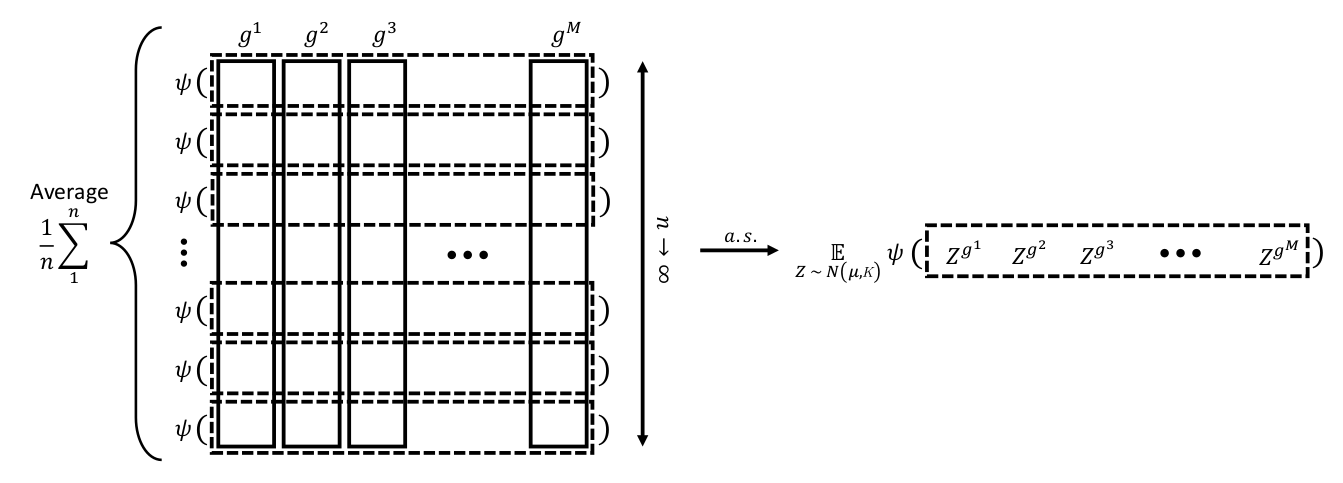
\includegraphics[width=\linewidth]{Figures/NETSOR_master_thm1.png}
	\caption{Illustration of Theorem \ref{thm:yangMaster}, from \cite{yang2019tensor}. If we suppose that $g^1, \dots, g^M$ are all the G-vars in a CDC (i.e. $g^{\mathfrak{c}} = (g^1, \dots, g^M)$), then, as the dimension $n$ increase, the empirical mean along the coordinates of the G-vars of an $\alpha$-controlled function $\psi$ converges to the expected value.
		Or, more intuitively, for each $i$, $(g^1_i, \dots, g^M_i) \approx \normdist(\mu, K)$.
	}
	\end{figure} 
	
	Intuitively, Theorem \ref{thm:yangMaster} states that $g_i^{\mathfrak{c}t} \stackrel{\text{d}}{\approx} \normdist(\mu^\mathfrak{c}, K^\mathfrak{c})$ for large $t$, iid for each $i$.
	This, jointly with the definitions of \eqref{eq:mean} and \eqref{eq:covariance}, means, roughly speaking, that the G-vars (preactivations, CFR Section \ref{subsec:tensorProg}) created from the same matrix $A^k$ have nonzero correlations, but otherwise are asymptotically independent unless they appear together in a LinComb.
	
	\subsection{Neural Tangent Kernel}\label{subsec:ntk}
	
	Has we have seen in Section \ref{subsec:iwl}, each neaural network architecture is equivalent, in the IWL to a Gaussian Process.
	This implies that we can study the regression we perform with the ANN as a kernel method, once we understand which kernel corresponds to its training.
	In this section, $\{x^i\}_{i\in [N]} \subset \R^{\text{dim}_\text{in}}$ denote the network inputs, $\theta \in \R^P$ contains all the parameters, distributed at initialization as in Section \ref{subsec:iwl}, and $f(\theta, x)$ is the output of the network, which, for notation simplicity, we suppose unidimensional.
	
	As in \cite{jacot2018neural} and \cite{arora2019exact}, we consider a training dataset $\{(x^i, y^i)\}_{i=1}^N \subset \R^{d_\text{in}} \times \R$ and we train the neural network by minimizing a convex loss function \[l(\theta) = \sum_{i=1}^N\mathcal{L}(f(\theta, x^i), y^i). \]
	We update the parameters at step $t$ using gradient descent with an infinitesimally small learning rate $\frac{d\theta(t)}{dt} = - \nabla l(\theta(t))$.
	With this setup, if we consider $l$ to be the mean squared error, by a simple differentiation \cite[Lemma 3.1]{arora2019exact} we see that the outputs of the network $u(t) = (f(\theta(t), x^i))_{i\in [N]}$ evolve according to 
	\begin{equation}\label{eq:dynamics}
		\frac{du(t)}{dt} = -\NTK(f_t) \cdot (u(t) - y),
	\end{equation}
	where $\NTK(f_t)$ is the $n \times n$ positive semidefinite matrix given by the \emph{Neural Tangent Kernel}.
	
	\definition{
		With the notation previously introduced, we define the \emph{Neural Tangent Kernel} $\NTK(\cdot, \cdot)$ as the kernel whose values on points $x, x'$ are given by 
		\begin{equation}\label{eq:ntk}
			\NTK(x, x') = \left\langle \frac{\partial f (\theta, x)}{\partial \theta}, \frac{\partial f (\theta, x')}{\partial \theta} \right\rangle. 
		\end{equation}
		As the values of $\theta$ are randomly initialized, we also define 
		\begin{equation}\label{eq:ntk_inf}
		\NTK_\infty(x, x') = \mathbb{E}_\theta [\NTK(x, x')].
		\end{equation}
		Finally, for any kernel $K$, we abuse the notation and, when the context make it clear, use $K$, or specifically $NTK$, to define the matrix whose entries $i,j$ are given by $K(x^i,x^j)$.
	}
	
	As we can see, the $\NTK$ depends on the parameters of the network and thus it is random at initialization and varies during training.
	Nonetheless, in \cite{jacot2018neural}, the authors prove that, if the ANN is an MLP, the $\NTK$ converges in the IWL to $\NTK_\infty$, which is ideed deterministic.
	Therefore, the dynamic expressed in \eqref{eq:dynamics} is identical to that of \emph{kernel regression} under gradient flow.
	
	It turns out that this idea is even more general.
	In fact, in \cite{jacot2018neural} Jacot et al. prove that the network function evolves along the kernel gradient given by the Neural Tangent Kernel for any convex loss function.
	We conjecture that this result holds true for any deep learning architecture.
	
	\subsection{Kernel Regression}\label{subsec:kernelRegression}
	
	Before moving to the experimental part, we remind the rider some concepts about \emph{kernel regression}.
	Suppose we have a kernel function $K(\cdot, \cdot)$ and a training dataset $\{(x^i, y^i)\}_{i=1}^N \subset \R^{d_\text{in}} \times \R$, kernel regression aims to approximate the underlying function with the linear combination
	\begin{equation}\label{eq:kernelReg}
		f(\cdot) = \sum_{i=1}^N \alpha^i K(\cdot, x^i).
	\end{equation}
	
	The coefficients are estimated to minimize the loss function over prediction points
	\begin{equation*}
		l(\alpha) = \mathcal{L}(f(x_*), y_*),
	\end{equation*}
	and in practice this minimization is carried over the training dataset
	\begin{equation}\label{eq:kernelCoeff}
		\widehat{\alpha} = \arg\inf\left\{\sum_{i=1}^N \mathcal{L}\left(\sum_{j=1}^N \alpha_j K(x^i,x^j), y^i\right) : \alpha_1,\dots, \alpha_N \in \R \right\}.
	\end{equation}
	
	\subsection{Multidimensional output}
	
	All we stated before about neural networks and kernels generalize immediately to the multi\-dimensional case upon noting that a function $f : \R^{d_\text{in}} \rightarrow \R^{d_\text{out}}$ is equivalent to a function $\tilde{f} : \R^{d_\text{in}} \times [d_\text{out}] \rightarrow \R$ with $\tilde{f}(x, k) = f_k(x)$.
	This said, we can generalize kernel regression, with each entry of the kernel $K(x, x')$ now being a matrix instead of a scalar and $\alpha$ being a vector, such that the vector-matrix product in \eqref{eq:kernelReg} produces indeed a vector output.
	In this case, the kernel matrix $K$ is a block matrix, where each block is given by the matrix $K(x^i, x^j)$.
	
	For the Neural Tangent Kernel, this means that 
	\begin{equation}\label{eq:multiNtk}
	[NTK(x^i,x^j)]_{k, k'} = \left\langle \frac{\partial f_k (\theta, x^i)}{\partial \theta}, \frac{\partial f_{k'} (\theta, x^j)}{\partial \theta} \right\rangle,
	\end{equation}
	with $k,k' \in [d_\text{out}]$.
	An interesting point of the multidimensional approach is that, as we can see in \eqref{eq:multiNtk}, the kernel also encodes information between different output coordinates, i.e. $k \neq k'$.
	
%	\section{Asymptotics results}\label{sec:asympthotics}
	
	\section{NTK implementation}\label{sec:implementation}
	
	\section{Experimental results}\label{sec:experiments}
	
	

%	\begin{figure}[h]
%		\begin{minipage}{0.5\textwidth}
%			\centering
%			\includegraphics[height=0.6\textwidth,width=0.75\textwidth]{example-image-a}
%		\end{minipage}
%		\begin{minipage}{0.5\textwidth}
%			\centering
%			\includegraphics[height=0.6\textwidth,width=0.75\textwidth]{example-image-a}
%		\end{minipage}
%		\captionof{figure}{Example of two \emph{zonotopes} in $\R^2$, generated by 3 and 4 line segments (in red).}
%	\end{figure}
%	
%	\begin{theorem}[Tizio and Caio, \cite{jacot2018neural}]
%		\begin{equation}\label{eq:Chak_Fill_3}
%		\Vol(\proj{I^n})\leq \sqrt{\frac{n!}{(n-k)!k!}}
%		\end{equation}
%	\end{theorem}
%
%	\definition{
%	Let $S = \veconeton \subset \R^k$.
%	\begin{itemize}	
%		\item We call $S$ an \emph{$(n,k)$-uframe} if there exist an orthonormal basis $\{\vec{f}_1,\ \ldots\ , \vec{f}_n\}$ of $\Rn$ such that for all $\vi\in S$ we have $\vi = \mathbf{P}(\vec{f}_i)$, where $\mathbf{P}$ denotes the orthogonal projection  from $\Rn$ to $\R^k$ .
%		\item We say that $S$ give a \emph{unit decomposition} if it satisfies
%		\begin{equation}
%		A_S|_{\R^k} = \sumin(\vi\otimes\vi)|_{\R^k}=\Id_k,
%		\end{equation}
%		where $\Id_k$ is the identity operator in $\R^k$.
%	\end{itemize}
%}
%
%	\begin{lemma}\label{lemma:t1}
%		\lipsum[23]
%	\end{lemma}
%	 \begin{proof}
%	 	\lipsum[7]
%	 	
%		 \begin{IEEEeqnarray*}{rCl}
%		 	A_s\tr & = & \sum_{\vec{v}\in S}(\vec{v}\otimes \vec{v})\tr = \sum_{\vec{v}\in S}\vec{v}\otimes \vec{v} = A_S, \\
%		 	\langle\vec{x}, A_S\vec{x}\rangle & = & \sum_{\vec{v}\in S}\langle\vec{x}, (\vec{v}\otimes \vec{v})\vec{x}\rangle = \sum_{\vec{v}\in S}\langle\vec{x},\vec{v}\rangle^2 \geq 0 \quad \forall\vec{x}\in \R^k,
%		 \end{IEEEeqnarray*}
%	\end{proof}
%
%	Looking at the structure of the matrix $A_S$, we see that
%	\begin{equation}\label{eq:A_S_Gram}
%	A_S[l,j] = \sumin(\vi\otimes\vi)[l,j] = \sumin(\vi[l]\vi[j]) = \langle M^S_l,M^S_j\rangle,
%	\end{equation}
%	
%	\begin{corollary}
%		The transformations on two vectors of $S$, namely $\vi$ and $\vj$, are, up to the sign, of the form :
%		\begin{IEEEeqnarray}{rCl}\label{eq:elliptic_rot}
%			\vip & = & \cos\alpha\:\vi - \sin\alpha\:\vj , \\
%			\vjp & = & \sin\alpha\:\vi + \cos\alpha\:\vj . \nonumber
%		\end{IEEEeqnarray}
%		We call the transformations of the form \eqref{eq:elliptic_rot} \emph{elliptic rotations}.
%	\end{corollary}
%	\begin{proof}
%		By Lemma \ref{lemma:t1}, the transformation $R$, in order to preserve all the vectors of $S$ aside $\vi$ and $\vj$, should modify, in $\Rn$, only $\ei$ and $\ej$ (i.e it should be a transformation of the 2-dimensional hyperplane spanned by those vectors). 
%%		 
%		Expressed in $\Span\{\ei,\ej\}$ coordinate system, $R$ is the composition of a rotation and a symmetry, so is given by
%		\[R = \left(\begin{array}{cc}
%			\ca & \sa \\ -\sa & \ca
%			\end{array}\right) 
%			\left(\begin{array}{cc}
%			 1 & 0 \\ 0 & -1
%			\end{array}\right)^r ,
%		\]
%		where $\ca = \cos\alpha$, $\sa=\sin\alpha$ and $r\in\{0,1\}$. Therefore, by linearity of the projection $\mathbf{P}$ onto $\R^k$ and dropping the symmetry part (as it does not influence the volume), we obtain the desired relation
%		\begin{IEEEeqnarray*}{rCl}
%		  	\mathbf{\mathbf{P}}(R\ei) & = & \mathbf{P}(\ca\ei -\sa\ej) = \ca \mathbf{P}(\ei)-\sa \mathbf{P}(\ej) = \ca\vi-\sa\vj = \vip , \\
%		  	\mathbf{P}(R\ej) & = & \mathbf{P}(\sa\ei +\ca\ej) = \sa \mathbf{P}(\ei)+\ca \mathbf{P}(\ej) = \sa\vi+\ca\vj = \vjp .
%		\end{IEEEeqnarray*}
%	\end{proof}

	\newpage
	\bibliographystyle{abbrv}
	\bibliography{References}
\end{document}